% Figure 3. Blowing up (printed page 29).
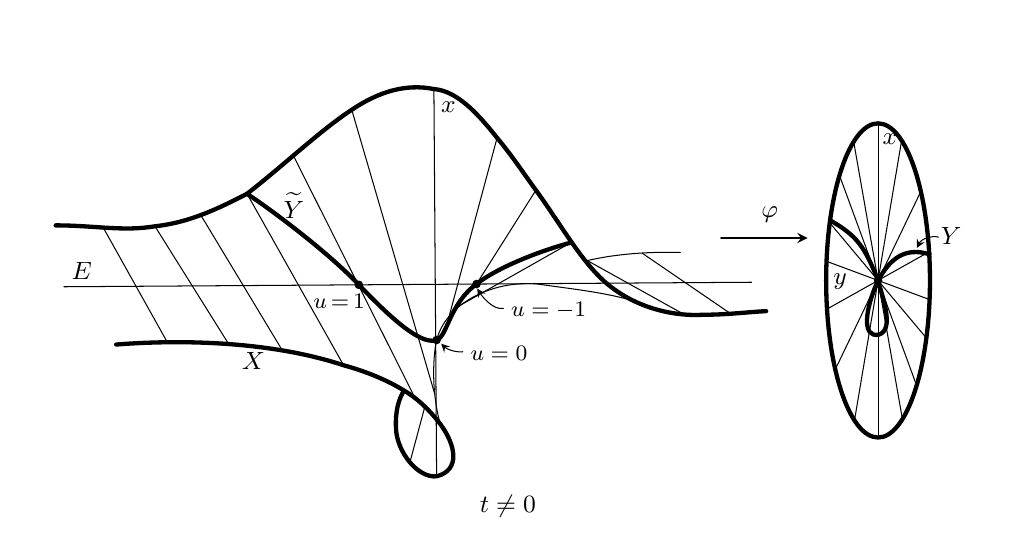
\begin{tikzpicture}[
    x=.325bp, y=-.325bp,
    line cap=round, line join=round, >=stealth,
    ruling/.style={line width=.37bp},
    contour/.style={line width=1.55bp},
    every node/.style={inner sep=0pt, font=\small}
  ]
  \path[use as bounding box] (-25,-14) rectangle (1048.846,535.538);

  \coordinate (turn) at (428,332);
  \coordinate (left-tip) at (218,170);
  \coordinate (right-tip) at (577,224);
  \coordinate (fold) at (392,388);

  % Exceptional curve, x-direction, and straight rulings on X.
  \draw[ruling] (15,273) -- coordinate[pos=.429] (positive)
    coordinate[pos=.600] (negative) (777,268);
  \draw[ruling] (425,54) -- (428,483);
  % The fold hides this ruling between its two visible pieces.
  \path (495,108) -- coordinate[pos=.600] (ruling-hidden)
    coordinate[pos=.824] (ruling-visible) (398,469);
  \draw[ruling]
    (59,208) -- (130,335)
    (116,206) -- (198,337)
    (167,194) -- (258,345)
    (left-tip) -- (325,360)
    (270,129) -- (405,398)
    (334,77) -- (426,392)
    (495,108) -- (ruling-hidden)
    (ruling-visible) -- (398,469)
    (538,166) -- (negative)
    (right-tip) -- (448,297)
    (595,244) -- (701,303)
    (656,236) -- (754,303);
  \draw[ruling]
    (fold) -- (384,405)
    (432,425) .. controls (422,389) and (424,350) .. (turn)
      .. controls (440,286) and (501,263) .. (547,271)
      .. controls (583,276) and (618,280) .. (647,289)
    (595,244) .. controls (625,237) and (660,234) .. (698,235);

  % Upper and lower rims of X, and the strict transform of Y.
  \draw[contour]
    (6,205) .. controls (49,205) and (81,212) .. (116,206)
    .. controls (154,202) and (187,186) .. (left-tip)
    .. controls (258,139) and (300,99) .. (334,77)
    .. controls (365,56) and (395,48) .. (425,54)
    .. controls (453,56) and (478,87) .. (495,108)
    .. controls (514,131) and (524,147) .. (538,166)
    .. controls (565,203) and (588,245) .. (616,269)
    .. controls (649,297) and (691,306) .. (724,304)
    .. controls (750,304) and (773,301) .. (793,300);
  \draw[contour]
    (73,337) .. controls (164,330) and (256,337) .. (325,360)
    .. controls (351,367) and (374,377) .. (fold)
    .. controls (409,398) and (423,413) .. (432,425)
    .. controls (449,448) and (455,476) .. (428,483)
    .. controls (407,485) and (384,456) .. (383,430)
    .. controls (382,411) and (386,397) .. (fold);
  \draw[contour]
    (left-tip) .. controls (251,192) and (310,237) .. (positive)
    .. controls (370,300) and (409,339) .. (turn)
    .. controls (440,328) and (442,292) .. (negative)
    .. controls (495,252) and (540,234) .. (right-tip);

  \fill (positive) circle[radius=1.55bp];
  \fill (negative) circle[radius=1.55bp];
  \fill (turn) circle[radius=1.55bp];
  \node at (441,74) {$x$};
  \node at (270,183) {$\widetilde{Y}$};
  \node at (35,256) {$E$};
  \node[font=\footnotesize] at (320,289) {$u\,{=}\,1$};
  \node[anchor=west,font=\footnotesize] at (510,299) {$u=-1$};
  \node[anchor=west,font=\footnotesize] at (465,347) {$u=0$};
  \node at (225,355) {$X$};
  \node at (507,516) {$t\ne 0$};
  \draw[ruling,->] (502,297)
    .. controls (490,299) and (478,283) .. (473,275);
  \draw[ruling,->] (457,345)
    .. controls (447,346) and (438,341) .. (433,336);

  \draw[->,line width=.65bp] (743,219) -- (839,219);
  \node at (797,193) {$\varphi$};

  % Target: the directions through the node of the plane cubic.
  \coordinate (O) at (917,266);
  \foreach \angle in {7,21.5,42,62,90,117,145.5,169.5} {
    \pgfmathsetmacro{\dx}{57.5*cos(\angle)}
    \pgfmathsetmacro{\dy}{174*sin(\angle)}
    \draw[ruling] (O) ++({-\dx},{-\dy}) -- ++({2*\dx},{2*\dy});
  }
  \draw[contour] (O) ellipse[x radius=57.5, y radius=174];
  \draw[contour]
    (864,199.5) .. controls (893,216) and (902,228) .. (O)
    .. controls (921,282) and (936,320) .. (918,326)
    .. controls (899,330) and (902,299) .. (O)
    .. controls (931,241) and (947,229) .. (974,237);
  \fill (O) circle[radius=1.55bp];
  \node at (930,110) {$x$};
  \node at (875,267) {$y$};
  \node[anchor=west] at (986,217) {$Y$};
  \draw[ruling,->] (984,218)
    .. controls (976,216) and (965,220) .. (960,230);
\end{tikzpicture}
